% For precision measurement of the physics processes at the LHC, an accurate
% description of the \gls{pdf} is important. The parton distribution functions are
% non-perturbative and extracted from global fit to hard-scatter data. Two kind of
% PDFs are considered:
% \begin{itemize}
% \item Intra-\gls{pdf} uncertainty: This is the uncertainty within a specific \gls{pdf}
%   set.
% \item Inter-\gls{pdf} uncertainty: This is the uncertainty when a certain
%   \gls{pdf} is replaced with another.
% \end{itemize}
% Three different groups provide equally precise parton distribution functions
% making it arbitrary to use one over the others to generate the signal MC
% samples. For this reason the recommendation of the PDF4LHC~\cite{PDF4LHC} group
% for a correct estimation of the \gls{pdf} uncertainty is to combine the
% uncertainties from all three groups and thus the CT10~\cite{CT10}, the
% NNPDF~\cite{NNPDF} and the MMHT~\cite{MMHT} \gls{pdf} sets have been used.

% The MC signal samples for the \gls{add} model are generated using the NNPDF set,
% in principle in order to evaluate the \gls{pdf} uncertainties for CT10 and MMHT
% it would be necessary to re-generate the signal samples using these \gls{pdf}
% sets. It is common practice to instead re-weight each event in the original
% sample to the value it would have if it were generated using an alternate PDF
% set. This is done using the LHAPDF~\cite{LHAPDF} tool.
% % The weight is given by:
% % \begin{equation}
% %   \label{eq:118}
% %   w = \frac{\mathrm{PDF}(x_1, f_1, Q) \cdot \mathrm{PDF}(x_2, f_2, Q)}
% %   {\mathrm{PDF}_0(x_1, f_1, Q) \cdot \mathrm{PDF}_0(x_2, f_2, Q)}
% % \end{equation}
% % where $\mathrm{PDF}$ is the alternate \gls{pdf} and $\mathrm{PDF}_0$ is the
% % \gls{pdf} used to generate the samples.

% The CT10 and the MMHT sets provide error sets to estimate the intra-\gls{pdf}
% uncertainty. The idea is that each \gls{pdf} has a number of uncorrelated
% parameters that can be varied independently by $\pm 1\sigma$ and a new \gls{pdf}
% can be calculated. This procedure is then repeated for each parameter in the
% \gls{pdf} set resulting in a set of \glspl{pdf}. This procedure is also done
% using the LHAPDF tool. The Hessian~\cite{Hessian} method is then used to
% estimate the uncertainty on the sets of \glspl{pdf}.

% For CT10 the symmetric Hessian method with 52 error sets is used where the
% uncertainty is given by:
% \begin{equation}
%   \label{eq:1190}
%   \delta X = \sqrt{\sum_{k = 1}^{n_\mathrm{err}} \left(X^{(k)} -
%       X^{(0)} \right)^2}
% \end{equation}
% where $X^{(0)}$ is the number of events using the best \gls{pdf} fit and
% $X^{(k)}$ is the number of events using the \gls{pdf} calculated varying the
% $k$-th parameter.

% For MMHT the asymmetric Hessian method with 50 error sets is used and the
% uncertainty is given by:
% \begin{align}
%   \label{eq:1200}
%     \delta x^{\mathrm{up}} & = \sqrt{\sum_{k = 1}^{n_\mathrm{err}/2}
%       \mathrm{max}(0, X_{2k} - X_0, X_{2k - 1} - X_0)^2} \\
%     \delta x^{\mathrm{down}} & = \sqrt{\sum_{k = 1}^{n_\mathrm{err}/2}
%       \mathrm{max}(0, X_0 - X_{2k}, X_0 - X_{2k - 1})^2}
% \end{align}
% where $X_0$ is the number of events obtained with the best fit and $X_{2k}
% (X_{2k -1})$ is the number of events calculated with the $2k$-th ($2k -1$-th)
% parameter variation.

% The NNPDF provides an ensemble of 100 \glspl{pdf} where the best value is given
% by the mean and the uncertainty by the standard deviation.
The \gls{add} signal sample is generated using the
\textsc{pythia8}~\cite{PYTHIA8} generator with the NNPDF2.3LO \gls{pdf} set. To
estimate the uncertainty deriving from the limited knowledge of the \glspl{pdf}
the same recommendations from the PDF4LHC group used in the estimation of the
\gls{pdf} uncertainties for the \gls{susy} compressed models and described in
\cref{sec:part-distr-funct} are used.

The \gls{pdf} uncertainties affects both the overall \gls{add} signal
normalization or cross section and the signal acceptance. \cref{fig:pdf_syst}
presents the observed variations in the number of signal \gls{add} events for
intra- and inter-\gls{pdf} uncertainties. The resulting relative yield
variations gives the relative \gls{pdf} uncertainty on the \gls{add} cross
section. The final \gls{pdf} uncertainty is the envelope that contains the error
bands of the three families.

\cref{tab:add_pdf_2016} summarizes the uncertainties on cross section and
acceptance. The growth of the uncertainty with both the number of extra
dimensions and the missing energy is understood with a similar argument as the
one given in \cref{sec:valid-effect-field}. Larger numbers of extra dimensions
require heavier gravitons (see \cref{fig:graviton_mass}) and thus a higher
center of mass energy of the originating partons. In these kinematic regions the
\glspl{pdf} are less well known. A similar argument can be used in the case of
higher $\met$ bins where higher momentum gravitons are produced.
\begin{figure}[!htb]
  \centering
  \begin{subfigure}{.48\linewidth}
    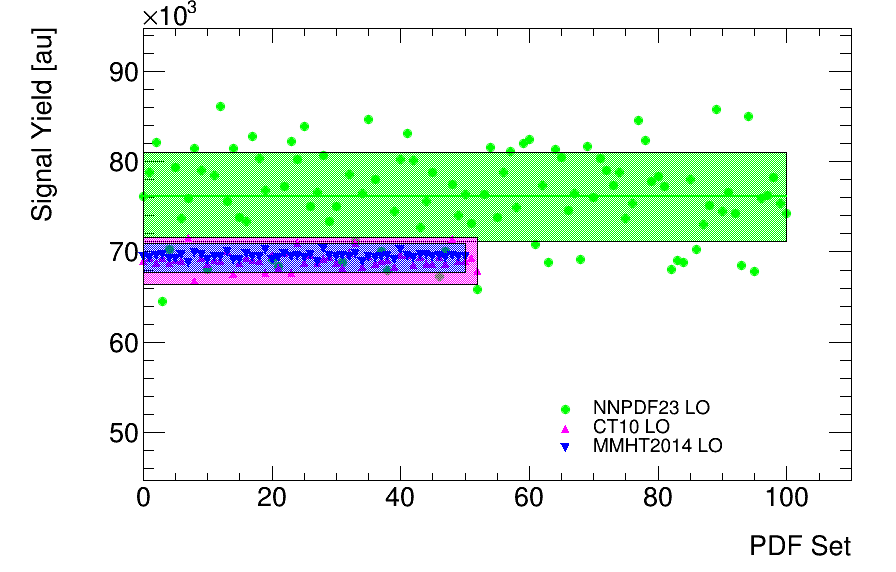
\includegraphics[width=\linewidth]{add_d2_MCut0_pdfset}
    \caption{ADD n = 2}
    \label{fig:pdf_n2}
  \end{subfigure}
  \begin{subfigure}{.48\linewidth}
    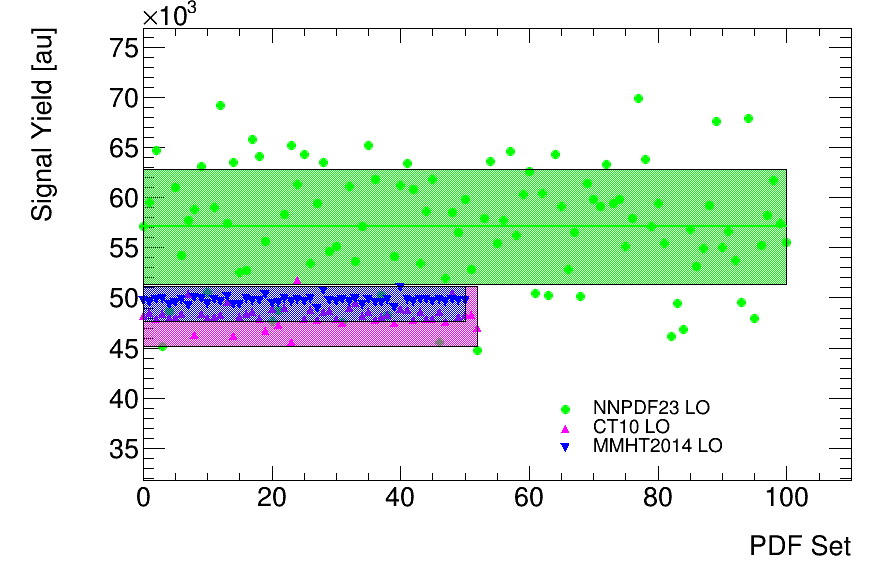
\includegraphics[width=\linewidth]{add_d3_MCut0_pdfset}
    \caption{ADD n = 3}
    \label{fig:pdf_n3}
  \end{subfigure}
  \begin{subfigure}{.48\linewidth}
    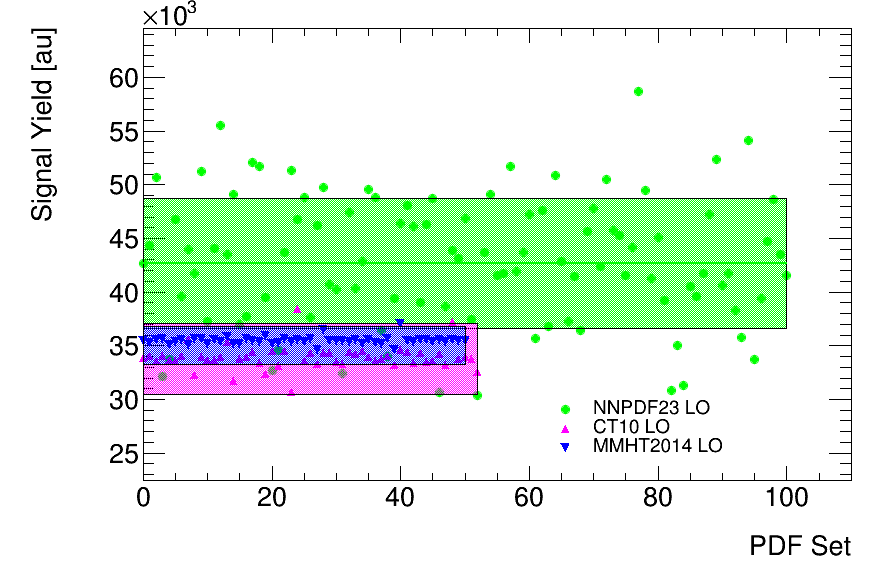
\includegraphics[width=\linewidth]{add_d4_MCut0_pdfset}
    \caption{ADD n = 4}
    \label{fig:pdf_n4}
  \end{subfigure}
  \begin{subfigure}{.48\linewidth}
    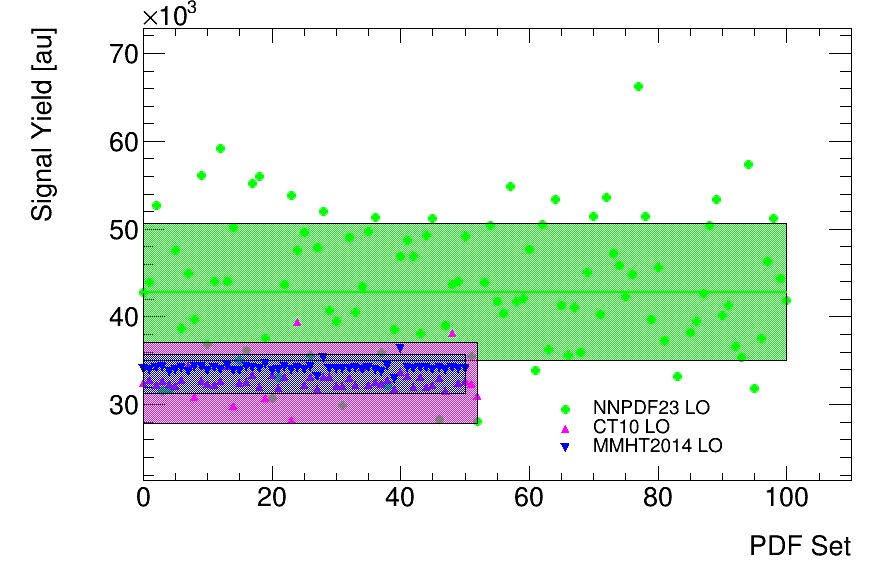
\includegraphics[width=\linewidth]{add_d5_MCut0_pdfset}
    \caption{ADD n = 5}
    \label{fig:pdf_n5}
  \end{subfigure}
  \begin{subfigure}{.48\linewidth}
    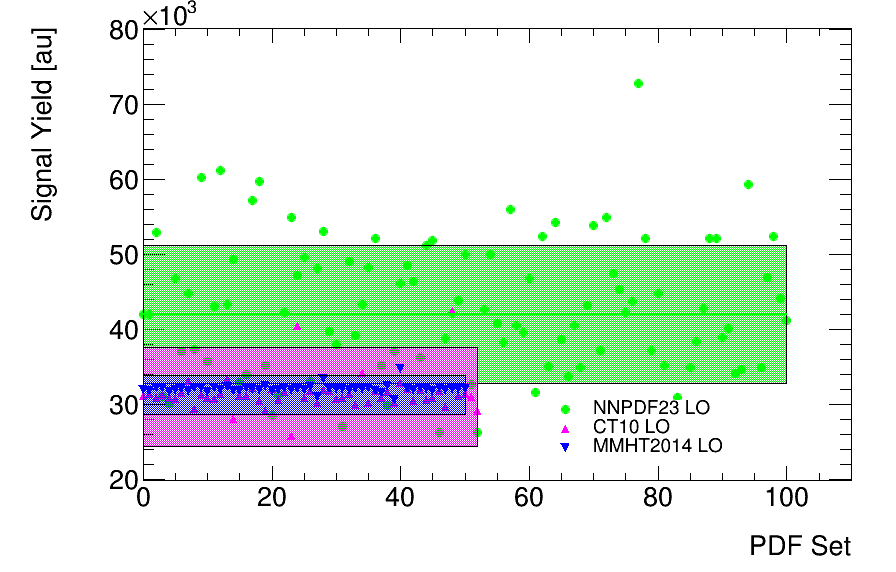
\includegraphics[width=\linewidth]{add_d6_MCut0_pdfset}
    \caption{ADD n = 6}
    \label{fig:pdf_n6}
  \end{subfigure}
  \caption{Observed variations in un-normalized number of \gls{add} events when
    the \gls{pdf} sets are varied by the uncertainties for n = 2 to n = 6. The
    event yield before any selection from three different \gls{pdf} families are
    compared. The final uncertainty on the \gls{add} cross section is the
    envelop that contains all three families with their error bands. The same
    procedure is also applied to the acceptances.}
  \label{fig:pdf_syst}
\end{figure}
\begin{table}[!h]
  \centering
  \resizebox{\linewidth}{!}{
  \begin{tabular}{lccccc}
    \toprule
    \multicolumn{6}{c}{PDF Uncertainty} \\
    \midrule \midrule
    \quad & ADD n = 2 & ADD n = 3 & ADD n = 4 & ADD n = 5 & ADD n = 6 \\
    \cline{2-6} \T
    $\Delta \sigma$ & 11 & 18 & 27 & 35 & 43 \\
    \midrule
    % $\Delta A (250 < \met < 300)$ & 4 & 8 & 10 & 11 & 17 \\
    % $\Delta A (300 < \met < 350)$ & 2 & 5 & 3 & 4 & 14 \\
    % $\Delta A (350 < \met < 400)$ & 5 & 7 & 3 & 1 & 8 \\
    $\Delta A (400 < \met < 500)$ & 8 & 11 & 12 & 13 & 13 \\
    $\Delta A (500 < \met < 600)$ & 13 & 13 & 15 & 11 & 14 \\
    $\Delta A (600 < \met < 700)$ & 16 & 16 & 18 & 20 & 8 \\
    $\Delta A (700 < \met < 800)$ & 18 & 21 & 19 & 15 & 20 \\
    $\Delta A (800 < \met < 900)$ & 21 & 19 & 20 & 12 & 9 \\
    $\Delta A (900 < \met < 1000)$ & 20 & 22 & 21 & 15 & 19 \\
    $\Delta A (\met > 1000)$ & 32 & 26 & 28 & 30 & 26 \\
    \bottomrule
  \end{tabular}}
  \caption{Systematic uncertainties in \% on \glspl{pdf}. The uncertainty is the
    envelop the contains the signal yields from the three \gls{pdf} families,
    plus their error bands.}
  \label{tab:add_pdf_2016}
\end{table}
%%% Local Variables:
%%% mode: latex
%%% TeX-master: "../search_for_DM_LED_with_ATLAS"
%%% End:
